\documentclass[wide,a4paper,titlepage,12pt] {article}
\usepackage{polski}
\usepackage{float}
\usepackage[utf8]{inputenc}
\usepackage{listings}
\usepackage{slashbox}
\usepackage[table]{xcolor}
\usepackage{graphicx,pdflscape}
\usepackage{placeins}


\title{Technologie sieciowe 2}
\author{Tymon Tobolski (181037)\\ Jacek Wieczorek (181043)}

% Title page layout (fold)
\makeatletter
\renewcommand{\maketitle}{
\begin{titlepage}
  \begin{center}
    \vspace*{3cm}
    \LARGE \@title \par
    \vspace{2cm}
    \textit{\small Autor:}\par
    \normalsize \@author\par \normalsize
    \vspace{3cm}
    \textit{\small Prowadzący:}\par
    Dr inż. Arkadiusz Grzybowski\par
    \vspace{2cm}
    Wydział Elektroniki\\ III rok\\ Pn TN 11.15 - 13.00\par
    \vspace{4cm}
    \small \@date
  \end{center}
\end{titlepage}
}
\makeatother


\begin{document}
\maketitle
  \section{Cel laboratorium}
  \paragraph{}
  Celem ćwiczenia jest zapoznanie się z oprogramowaniem GnuPG do szyfrowania i odpisywania dokumentów elektronicznych oraz zarządzaniem kluczami. W ramach ćwiczenia student zapoznaje sie z: podstawowymi algorytmami kryptograficznymi, tworzeniem, eksportem i importem kluczy, podpisywaniem e-maili oraz plików, budowaniem sieci zaufania.

  \section{Zadania}
  \paragraph{}

  \subsection{Generowanie kluczy}
  \paragraph{}
  Klucz GPG można utworzyć z lini komend wydając polecenie \texttt{gpg --gen-key}.
  Podczas generowania program pyta użytkownika o szereg opcji:

  \begin{itemize}
    \item Typ szyfrowania - RSA, DSA
    \item Długość klucza - od 1024 do 4096 bitów
    \item Czas ważności klucza
    \item Dane właściciela klucza - imie i nazwisko, adres email oraz opcjonalny komentarz
  \end{itemize}

  \paragraph{}
  Ostatnim etapem generowania klucza jest dwukrotne podanie hasła zabezpieczającego klucz.

  \paragraph{}
  Rysunek 1 pokazuje generowanie klucza z szyfrowaniem RSA, o długości klucza 1024 bitów, ważnego przez 4 dni.

  \begin{figure}[h!]
    \begin{center}
      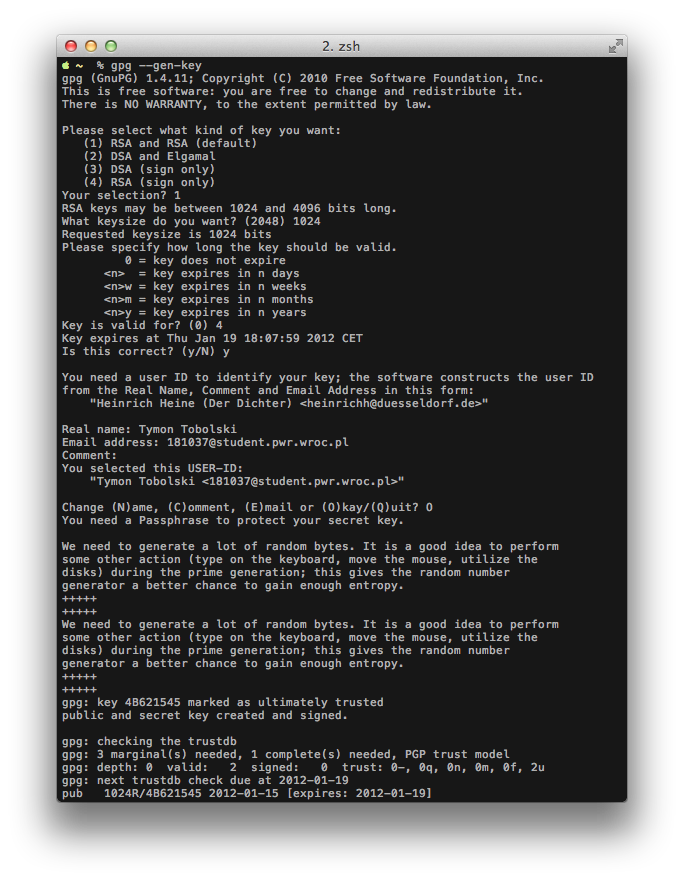
\includegraphics[width=\textwidth]{img/1.png}
      \caption{Generowanie klucza GPG}
    \end{center}
  \end{figure}

  \newpage
  \paragraph{}
  \newpage

  \subsection{Dodawanie, usuwanie i modyfikacja kluczy}
  \paragraph{}
  W celu wyświetlenia listy wygenerowanych kluczy można użyć polecenia \texttt{gpg --list-keys}.

  \begin{figure}[h!]
    \begin{center}
      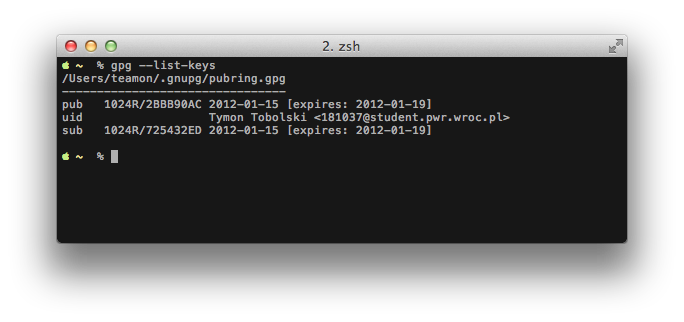
\includegraphics[width=\textwidth]{img/2.png}
      \caption{Wyświetlenie listy kluczy}
    \end{center}
  \end{figure}

  \paragraph{}
  Edycji klucza można dokonać przy pomocy polecenia \texttt{gpg --edit-key NAZWA}. Rysunek 3 pokazuje proces edycji klucza o nazwie $"Tymon\ Tobolski\ <181037@student.pwr.wroc.pl>"$. W tym wypadku został zmieniony termin ważności klucza na 2 miesiące przy użyciu komendy \texttt{expire}. W celu sprawdzenia wszysktich dostępnych komend można wykorzystać polecenie \texttt{help} Przy zapisie zmian program wymaga podania hasła zabezpieczającego klucz.


  \begin{figure}[h!]
    \begin{center}
      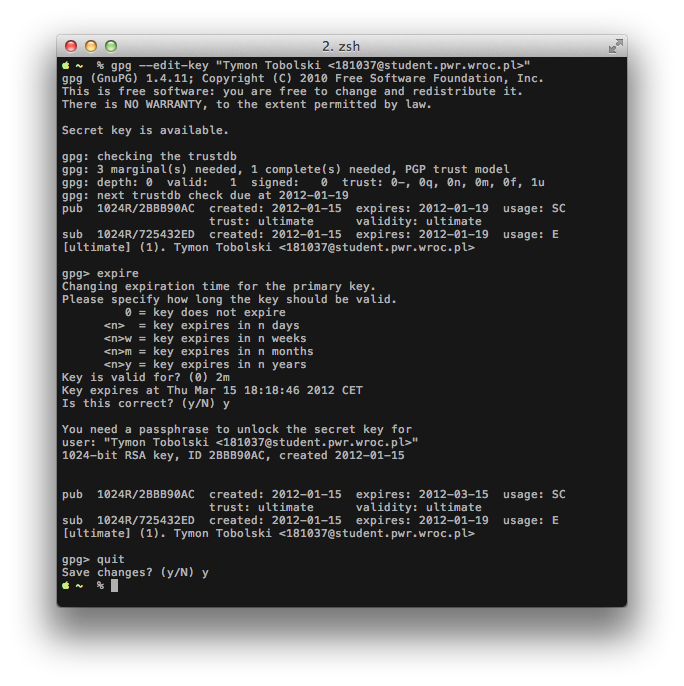
\includegraphics[width=\textwidth]{img/3.png}
      \caption{Edycja klucza}
    \end{center}
  \end{figure}

  \newpage
  \paragraph{}
  \newpage

  \paragraph{}
  W celu usunięcia klucza należy najpierw usunąć klucz prywatny przy pomocy polecenia \texttt{gpg --delete-secret-key NAZWA}, a następnie usunąc klucz publiczny za pomocą komendy \texttt{gpg --delete-key NAZWA}. Samo usunięcie klucza prywatnego nie powoduje skosowania użytkownika. Nie jest możliwe usunięcie tylko klucza publicznego.


  \begin{figure}[h!]
    \begin{center}
      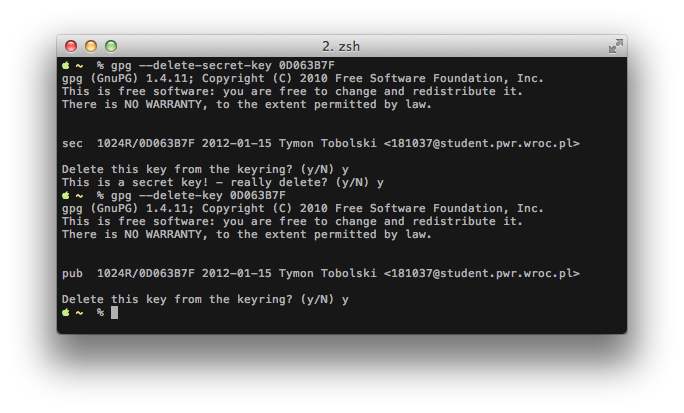
\includegraphics[width=\textwidth]{img/4.png}
      \caption{Usunięcie klucza}
    \end{center}
  \end{figure}

  \newpage

  \subsection{Unieważnienie klucza}
  \paragraph{}
  Unieważnienie klucza możliwe jest w trybie edycji za pomocą komendy \texttt{revkey}. Rysunek 5 przedstawia przykład unieważnienia klucza za pomocą programu gpg. Podczas procesu uniważnienia można opcjonalnie podać przyczyne oraz komentarz. Wymagane jest również podanie hasła zabezpieczającego dany klucz.


  \begin{figure}[h!]
    \begin{center}
      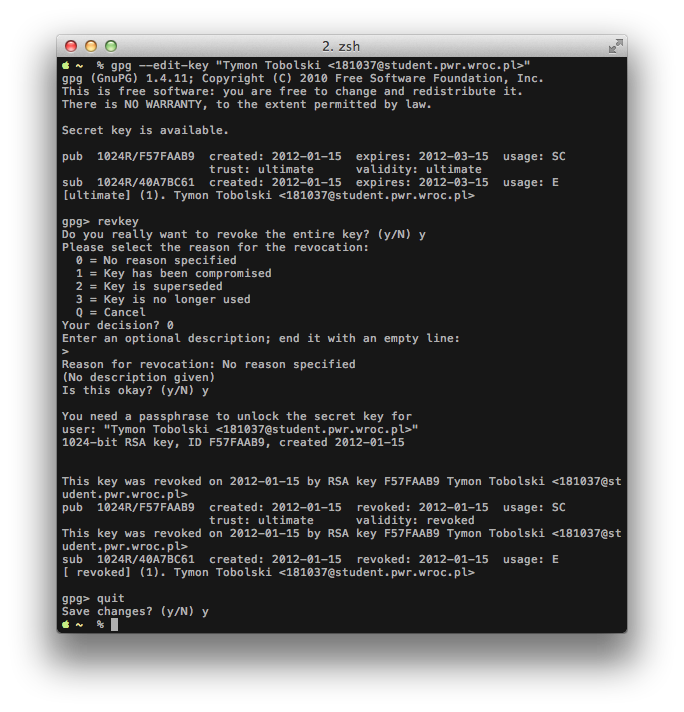
\includegraphics[width=\textwidth]{img/5.png}
      \caption{Unieważnienie klucza}
    \end{center}
  \end{figure}

  \subsection{Eksport i import kluczy}
  \paragraph{}
  Eksport klucza publicznego jak i prywatnego sprowadza się do wywołania 2 komend: \texttt{gpg --export -a NAZWA} dla klucza publicznego oraz \texttt{gpg --export-secret-key -a} dla klucza prywatnego. Rysunki 6 i 7 pokazują wynik działania tych komend.

  \begin{figure}[h!]
    \begin{center}
      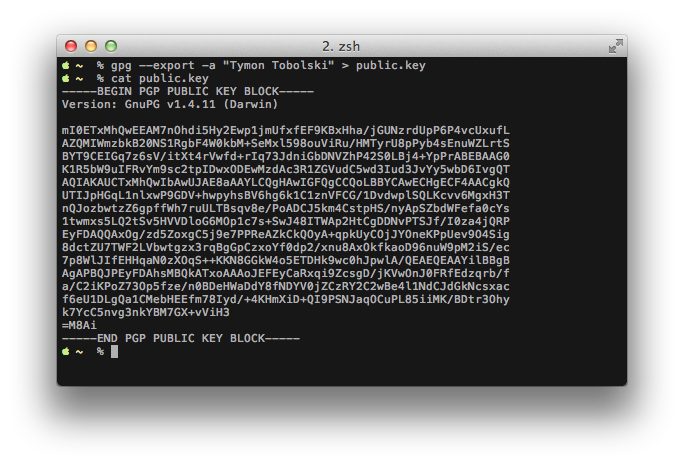
\includegraphics[width=\textwidth]{img/6.png}
      \caption{Eksport klucza publicznego do pliku}
    \end{center}
  \end{figure}

  \begin{figure}[h!]
    \begin{center}
      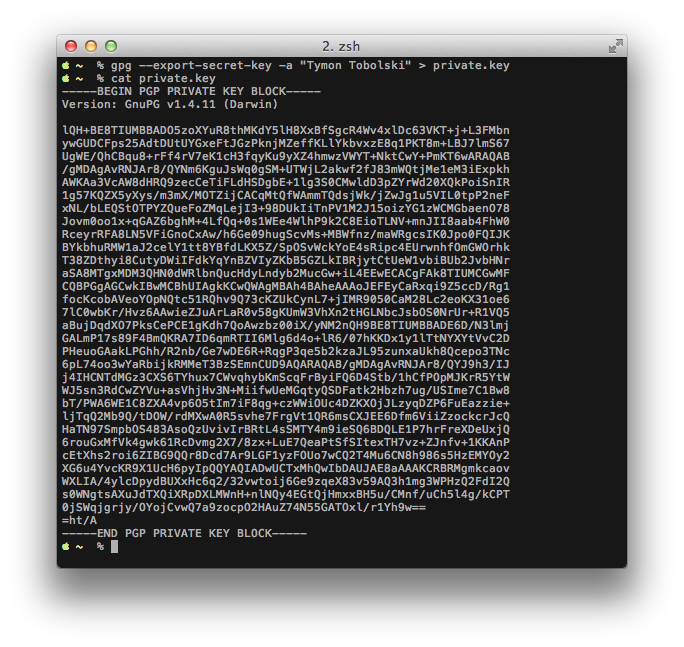
\includegraphics[width=\textwidth]{img/7.png}
      \caption{Eksport klucza prywatnego do pliku}
    \end{center}
  \end{figure}

  \newpage


  \paragraph{}
  Po wyeksportowaniu klucza publicznego do pliku, można go przesłać innemu użytkownikowi. Może on wtedy zaimportować klucz i podpisać go za pomocą swojego własnego. W celu podpisania klucza przy użyciu programu gpg należy wejść w tryb edycji klucza, a następnie wywołać polecenie \texttt{sign}. Następnie należy podać hasło zabezpieczające klucz, którym podpisany będzie klucz .Rysunki 8 i 9 przedstawiają operacje importu oraz podpisywania klucza.

  \begin{figure}[h!]
    \begin{center}
      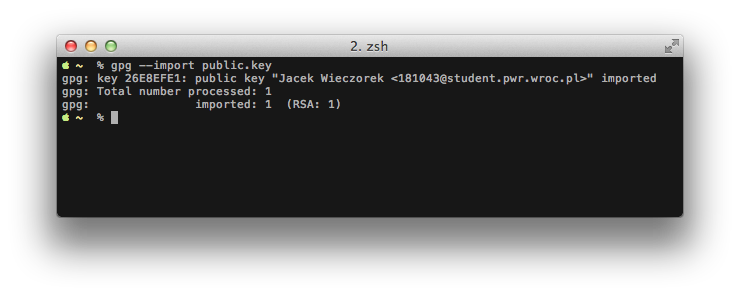
\includegraphics[width=\textwidth]{img/8.png}
      \caption{Import klucza z pliku}
    \end{center}
  \end{figure}

  \begin{figure}[h!]
    \begin{center}
      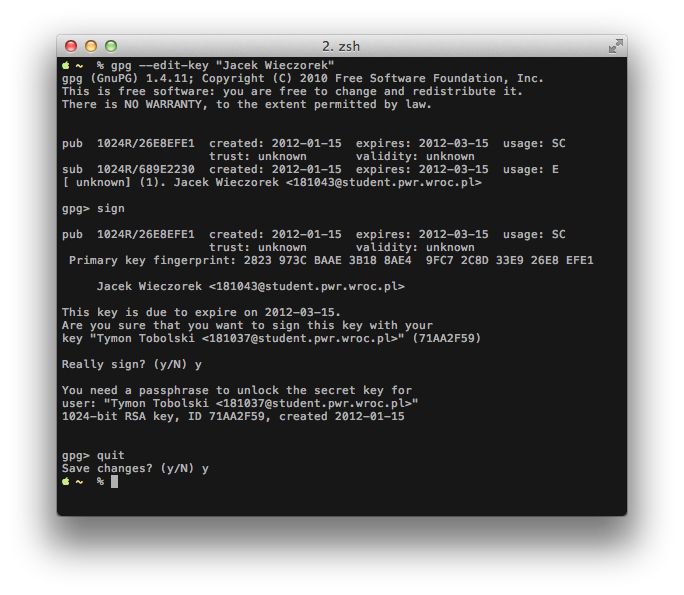
\includegraphics[width=\textwidth]{img/9.png}
      \caption{Podpisanie klucza}
    \end{center}
  \end{figure}

  \paragraph{}
  Budowanie sieci zaufania może okazać się czasochłonne, ze względu na konieczność wymiany kluczy między użytkownikami.

  \newpage

  \section{Wykorzystanie serwerów kluczy}
  \paragraph{}
  Wysłanie klucza na serwer wymaga podania adresu serwera, odbywa się za pomocą komendy \texttt{gpg --keyserver SERWER --send-keys ID\_KLUCZA}. Rysunek 10 przedstawia proces wysłania klucza na serwer pgp.mit.edu.

  \begin{figure}[h!]
    \begin{center}
      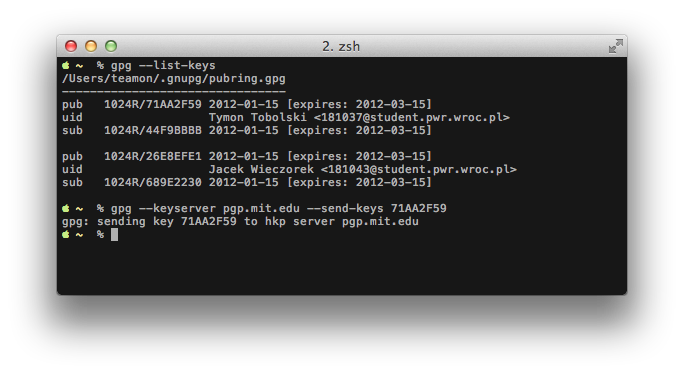
\includegraphics[width=\textwidth]{img/10.png}
      \caption{Przesłanie klucza na serwer pgp.mit.edu}
    \end{center}
  \end{figure}

  \paragraph{}
  Serwer kluczy udostępnia możliwość wyszukiwania kluczy na dwa sposoby: za pomocą identyfikatora klucza (\texttt{gpg --keyserver SERWER --search-key ID\_KLUCZA}) lub poprzed adres email (\texttt{gpg --keyserver SERWER --search-key EMAIL}). Rysunek 11 przedstawia obie metody wyszukiwania klucza na serwerze pgp.mit.edu.

  \begin{figure}[h!]
    \begin{center}
      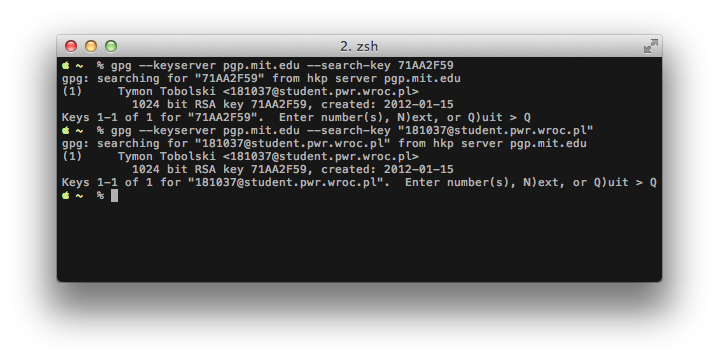
\includegraphics[width=\textwidth]{img/11.png}
      \caption{Wyszukiwanie klucza na serwerze pgp.mit.edu}
    \end{center}
  \end{figure}

  \paragraph{}
  Serwery kluczy znacznie usprawniają wymiane kluczy między użytkownikami. Każdy może zapytać serwer o klucz publiczny podanego adresu email, nie ma potrzebu wysyłania go do każdego użytkownika z osobna.

  \subsection{Szyfrowanie, deszyfrowanie, podpisywanie i weryfikacja podpisu plików}
  \paragraph{}
  Podpisywanie plików dobywa się za pomocą komendy \texttt{gpg --clearsign PLIK}. Podpis pliku wymaga podania hasła zabezpieczającego klucz. Po podpisaniu pliku zostaje utworzony plik z podpisem o rozszerzeniu .asc  Przyład takiego podpisu prezentuje Rysunek 12.

  \begin{figure}[h!]
    \begin{center}
      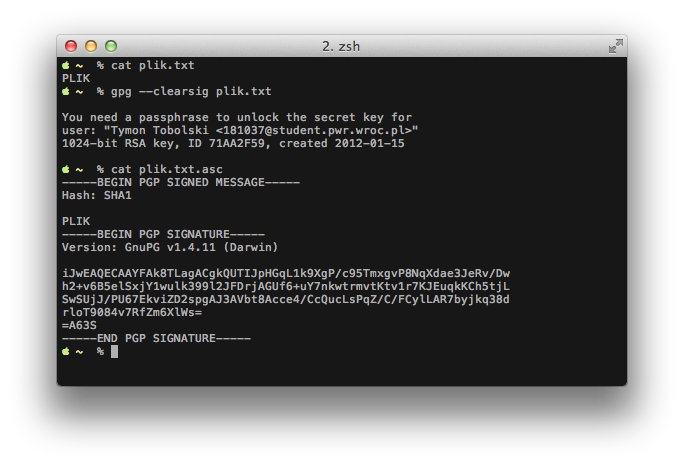
\includegraphics[width=\textwidth]{img/12.png}
      \caption{Podpisywanie pliku}
    \end{center}
  \end{figure}

  \paragraph{}
  Weryfikacji podpisu można dokonać przy pomocy komendy \texttt{gpg --verify PLIK\_ASC}. Przykładowa operacja zaprezentowana jest na Rysunku 13.

  \begin{figure}[h!]
    \begin{center}
      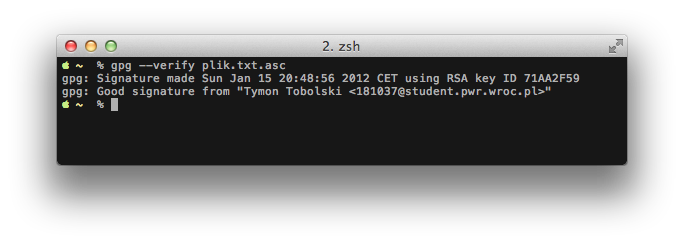
\includegraphics[width=\textwidth]{img/13.png}
      \caption{Weryfikacja podpisu pliku}
    \end{center}
  \end{figure}

  \paragraph{}
  W celu zaszyfrowania wiadomości należy wywołać komende \texttt{gpg --recipient ODBIORCA --output PLIK\_GPG --encrypt PLIK}. Po zaszyfrowaniu powstaje plik .gpg. Przyład szyfrowania wiadomości znajduje się na Rysunku 14.

  \begin{figure}[h!]
    \begin{center}
      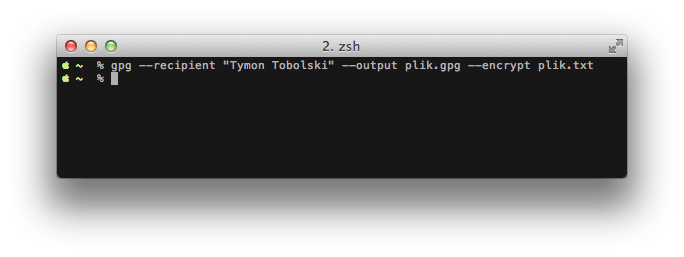
\includegraphics[width=\textwidth]{img/14.png}
      \caption{Szyfrowanie wiadomości}
    \end{center}
  \end{figure}

  \paragraph{}
  Deszyfracja wiadomości sprowadza się do wykonania komendy \texttt{gpg --decrypt-files PLIK\_GPG}. Ta operacja wymaga podania hasła zabezpieczającego klucz. Przykład użycia obrazuje Rysunek 15.

  \begin{figure}[h!]
    \begin{center}
      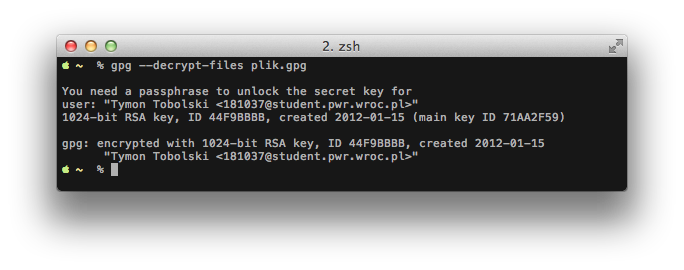
\includegraphics[width=\textwidth]{img/15.png}
      \caption{Szyfrowanie wiadomości}
    \end{center}
  \end{figure}

\end{document}
